\documentclass[12pt, letterpaper]{article}
\usepackage{bbold}
\usepackage{indentfirst}
\usepackage{amsmath, amssymb}
\usepackage[T1]{fontenc}
\usepackage[utf8]{inputenc}
\usepackage{physics}
\usepackage{tensor}
\usepackage{braket}
\usepackage{graphics}
\usepackage{grffile}
\usepackage[export]{adjustbox}
\usepackage{svg}
\usepackage{caption}
\usepackage{subcaption}
\usepackage{authblk} 
\usepackage{blindtext}
\usepackage{setspace}
\usepackage{xcolor}
\usepackage{tcolorbox}
\usepackage{listings}
\usepackage[framemethod=TikZ]{mdframed}
\mdfdefinestyle{MyFrame}{%
    linecolor=black,
    outerlinewidth=2pt,
    roundcorner=20pt,
    innertopmargin=\baselineskip,
    innerbottommargin=\baselineskip,
    innerrightmargin=20pt,
    innerleftmargin=20pt,
    backgroundcolor=gray!50!white}
\title{}

\begin{document}
    \section*{Report On Using MCMC Method To Find Hamiltonian And Thermalizaion of Berry-Keating And Damped Harmonic Oscillator}
    \subsection*{Preliminaries}
        Hamiltonian of Berry-Keating  
        \begin{equation}
            H = \frac{1}{2}(xp + px)
        \end{equation}
        \\
        
    

        We're using MCMC method to evaluate Hamiltonian and Thermalization of Berry-Keating. 
    
    \subsection*{Methodology}
        Markov Chain Monte Carlo (MCMC) is a random sampling method to visit x with a probability proportional to some given
        distribution say, $\pi (x)$. To use MCMC in simulation we first simplify the Hamiltonian Monte Carlo code in a block
        manner. Then we calculate and plot $<H>$ graphs of Berry-Keating Hamiltonian. 
        But first simplify code using header files. Those codes are giiven below

        \begin{adjustbox}{center,caption={Graph of Expectation value of Berry-Keating},nofloat=figure,label={somelabel}}
            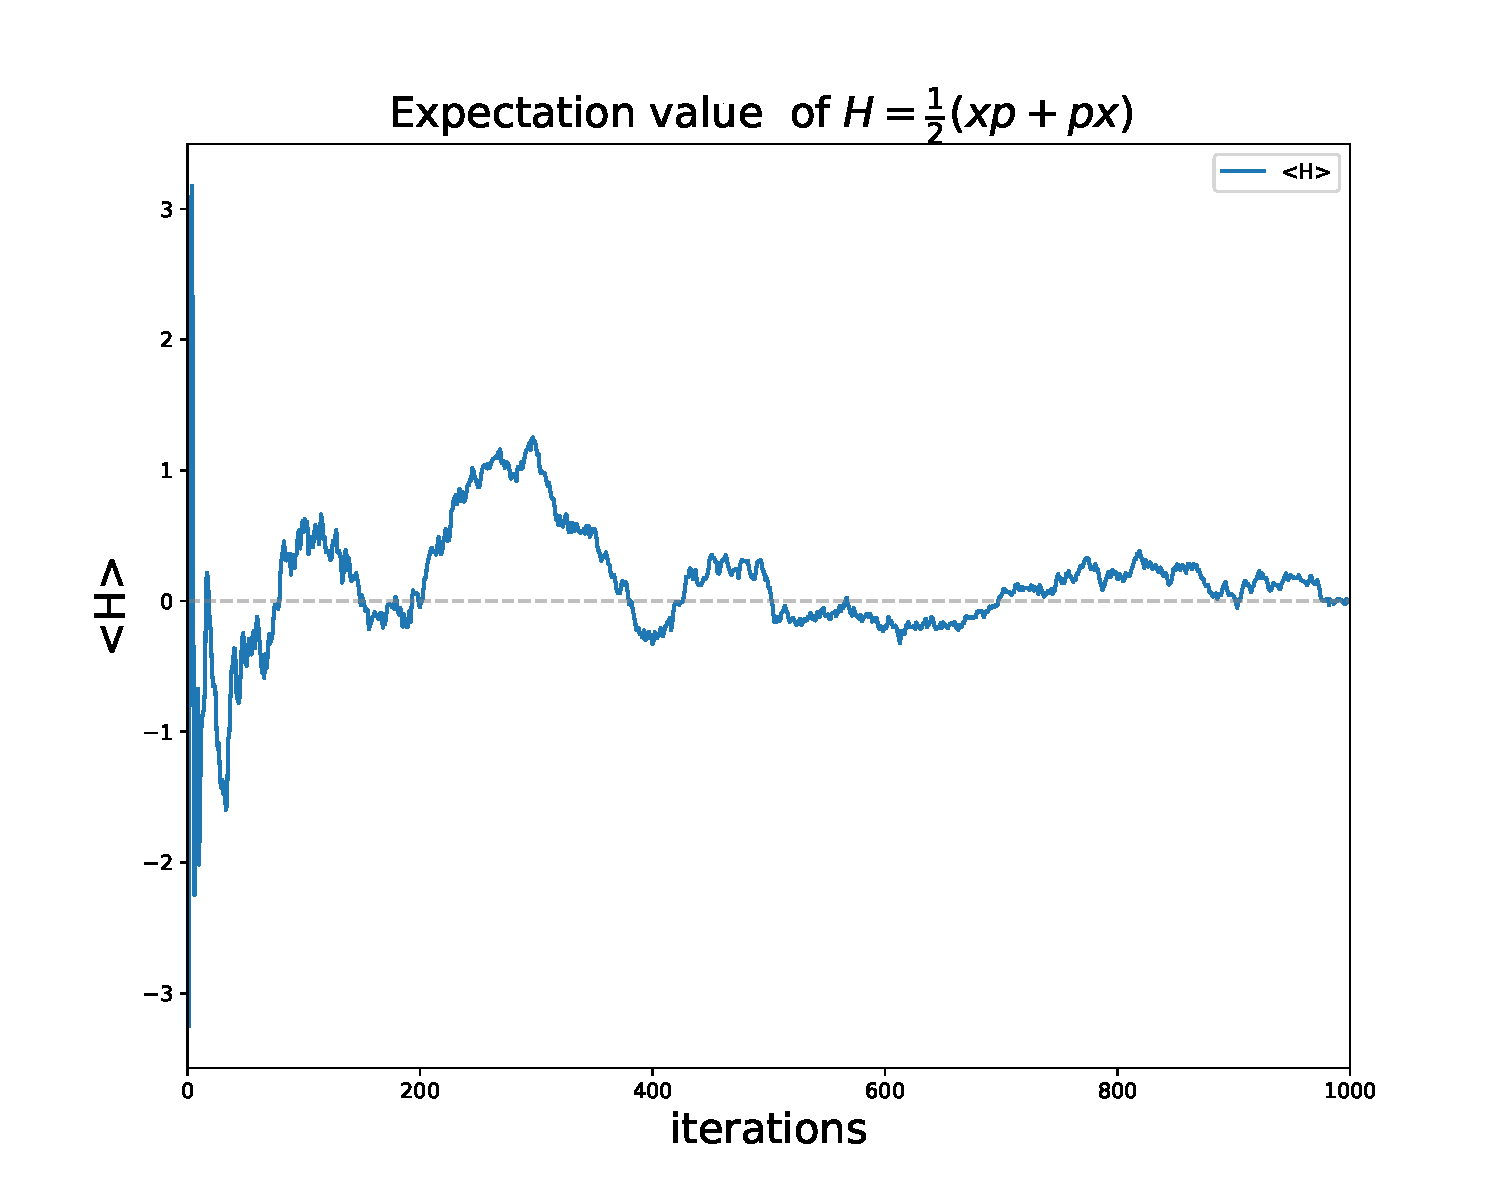
\includegraphics[width=0.8\textwidth]{bk.pdf}
        \end{adjustbox}

        Again evaluating $<H>$ using probability function where

        \begin{equation}
            <H> = Tr (\frac{\hat{H}*exp(-\beta \hat{H})}{Tr (exp(-\beta \hat{H} ))})
        \end{equation}
        \begin{adjustbox}{center,caption={Graph of Expectation value of Berry-Keating},nofloat=figure,label={somelabel}}
            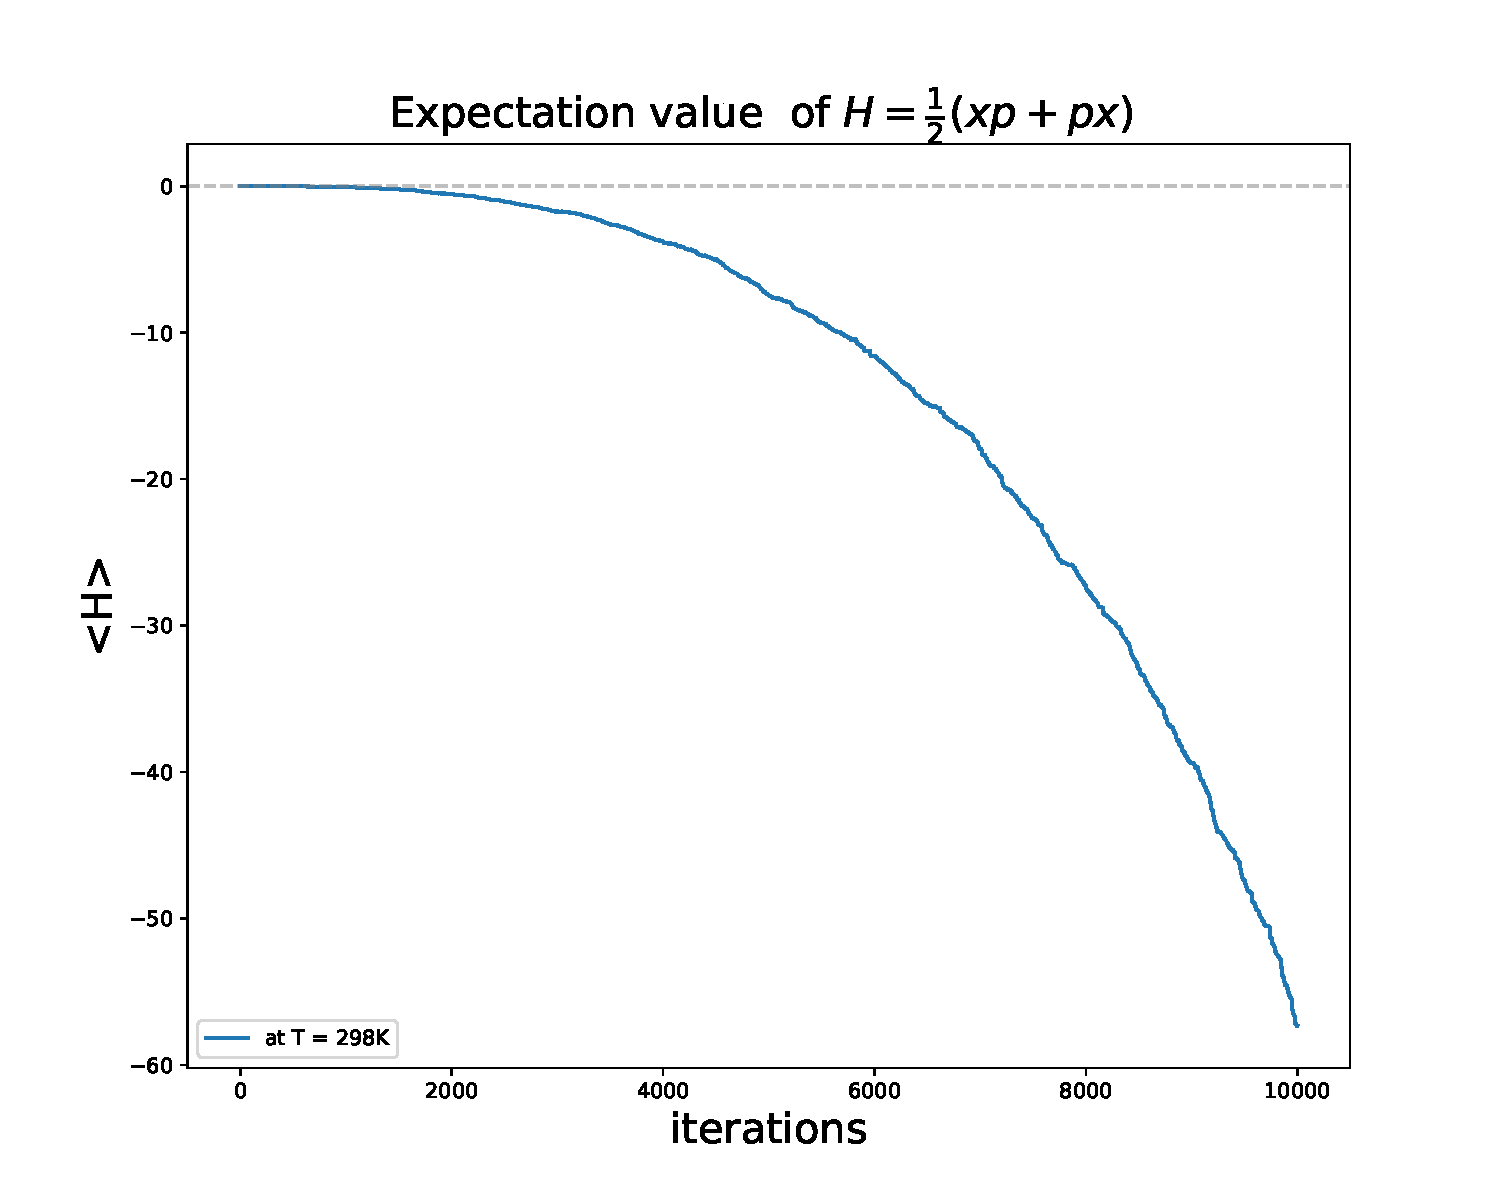
\includegraphics[width=0.8\textwidth]{beta.pdf}
        \end{adjustbox}
\end{document}